%% This is an example first chapter.  You should put chapter/appendix that you
%% write into a separate file, and add a line \include{yourfilename} to
%% main.tex, where `yourfilename.tex' is the name of the chapter/appendix file.
%% You can process specific files by typing their names in at the 
%% \files=
%% prompt when you run the file main.tex through LaTeX.
\chapter{Introduction}

Finding a route with the least travel time on a large road network in a metropolis is not only of algorithmic interests, but also of economic and environmental values. Less travel time means less fuel consumptions and less carbon emissions. However, finding the \emph{shortest} route can be a challenging task, especially when the road traffic is known to be \emph{time-dependent} or \emph{dynamic}, namely, when the travel cost changes with respect to time. It may take 10 minutes on average to traverse a particular road at 10~a.m., but it is possible that the expected travel time increases to 20 minutes at 5~p.m. Moreover, the travel costs of two different roads may have different time-varying patterns. For instance, one road may have a peak travel time at 12~p.m. but the other may have two peaks at 8~a.m. and 6~p.m., respectively. Definition~\ref{Def: road_net} gives a formal description of a dynamic road network, based on which the generalised time-dependent shortest path problem is defined in Definition~\ref{Def: shortest_path_problem}.

\begin{defn}[\emph{Dynamic road network}]\label{Def: road_net}
A dynamic road network is a weighted, directed graph $G=(V,E)$ where $E$ represents a set of road segments and $V$ denotes the set of intersections amongst the road segments. It has a weight function $w : E,t \rightarrow \mathbb{R}$, where $t$ represents a moment in time. 
\end{defn}

\begin{defn}[\emph{Generalised time-dependent shortest path problem}]\label{Def: shortest_path_problem}
In a dynamic road network $G=(V,E)$, given a source node $u$, a destination node $v$ and a departure time $t$ from $u$, find a path $p$ that satisfies:
\begin{equation}
w(p)=\delta(u,v)=
\begin{cases}
\text{min}\left\{w(p): u\overset{p}{\leadsto}v \right\} &\text{if there is a path from $u$ to $v$,}\\
\infty &\text{otherwise.}
\end{cases}
\end{equation}
where $w(p)$ is the weight of the path $p$ and defined as sum of the weights of its constituent edges, and $\delta(u,v)$ is known as the \textbf{shortest-path weight} from $u$ to $v$.
\end{defn}

A typical Bellman-Ford \cite{CLRS09} or Dijkstra's algorithm \cite{Dij59} for finding shortest paths assume the cost of traversing each edge in a graph is constant with respect to time and therefore, do not work on time-de\-pendent road networks without appropriate modifications. Fortunately, most online mapping services such as Google Maps or Baidu Maps are able to recommend shortest routes by interpolating real-time traffic information. This project seeks to investigate an alternative approach of finding shortest routes on a dynamic road network based on mining a GPS\footnote{Global Positioning System} trajectory database aggregated from thousands of taxis in Beijing, China.

Chapter~\ref{Chap:2} describes the steps taken in preliminary data processing, where outliers in the data set are removed and each GPS trajectory is mapped to a set of streets. Chapter~\ref{Chap:3} introduces the approach for constructing a landmark graph that represents a city's road network in an abstract way. Chapter~\ref{Chap:4} discusses the method to estimate the travel cost of each edge in a landmark graph. Chapter~\ref{Chap:5} presents an algorithm for finding a shortest path given the dynamic travel costs. 

\section{Motivations for Mining Taxi GPS Trajectories}
Taxi drivers or any experienced car drivers, more often than not, possess some \emph{implicit} knowledge or intuitions about which route from a source $u$ to a destination $v$ is the best in terms of travel time at a particular moment. Such knowledge or intuitions stem from everyday experiences. For example, a taxi driver may observe that there are always traffic jams from 6~p.m. to~7 p.m. on a particular street and hence avoid travelling on that street during that period of time whenever possible. But observations of this kind, albeit valuable, are too subtle to be captured by any general algorithms and oftentimes, even drivers themselves may not be fully aware of that.

However, mining their GPS trajectories can be an excellent way of revealing such knowledge. In a metropolis such as Beijing or New York, taxi drivers are required by regulations to install GPS devices on their cars and to send time-stamped GPS information to a central reporting agency periodically, for management and security reasons. The GPS information typically includes latitudes, longitudes, instantaneous speeds and heading directions. Therefore, such GPS data is readily available and little effort is needed to collect it. By means of mapping to a real road network all GPS data points pertaining to a particular taxi during a specific period of time, a GPS trajectory can be obtained to represent the driver's intelligence. Definition~\ref{Def: trajectory} formally defines taxi trajectories. 

\begin{defn}[\emph{Taxi Trajectory}]\label{Def: trajectory}
A taxi trajectory $T = (p_1,p_2,\textellipsis,p_n)$ is a set of chronologically ordered GPS data points pertaining to one taxi. The time span between $p_1$ and $p_n$ is defined as the \emph{duration} of the trajectory. 
\end{defn}

\section{Practical Limitations} \label{Sec:limitation}
Some practical limitations are worth mentioning. 
\subsubsection{Arbitrary sources and destinations}
In a typical map-query use case, a user is able to select an arbitrary source to start with and an arbitrary destination to go to. But this may not be possible for the approach proposed in this project, since the taxi GPS trajectories do not necessarily cover every part of a city's road network. It is likely that there are no trajectories passing through one particular source and one particular destination.

\subsubsection{Low sampling rate}
Taxis report their locations to the central reporting agency at a relatively low frequency to conserve energy. For the data set used in this project, the expected sampling interval is one minute. But oftentimes, the GPS device may not be working properly or may be occasionally shut down due to various reasons, which causes the actual sampling interval to fluctuate. 

Even if the sampling interval \emph{is} strictly kept at one minute, for a taxi moving at a typical speed of $60 km/h$, it means the distance between two consecutive sample points is $1 km$. Such a large distance increases the uncertainty about the \emph{exact} trajectory that the taxi has moved along. Figure~\ref{Fig:low_sampling_rate} \cite{TDR10} demonstrates a problem caused by low sampling rate and long inter-sample-point distance.
\begin{figure}[h!]
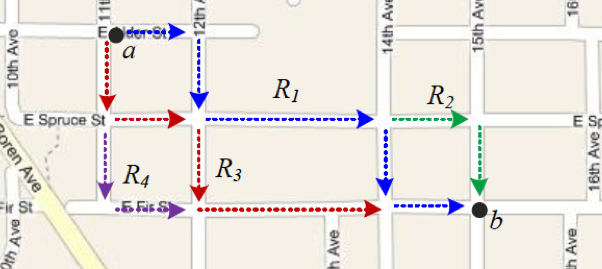
\includegraphics{low_sample_rate}
\centering
\caption{An example of low-sampling-rate problem}
\label{Fig:low_sampling_rate}
\end{figure}

The taxi is known to have traversed from point $a$ to point $b$. But there are four possible trajectories from $a$ to $b$. In this case, the exact route cannot be determined without additional information.

\subsubsection{Limited GPS accuracy}
After decades of development, the GPS has achieved great accuracy, but it is not completely error-free. A report \cite{FP15} in 2015 showed that GPS-enabled smartphones typically have an accuracy of 5 metres \emph{under open sky}. But in a metropolis like Beijing, the actual accuracy may be lower due to the reflection of signals amongst high buildings. Moreover, the data set used in this project was collected in 2009 when GPS devices had lower accuracy than they have today.

The limited accuracy in GPS devices makes the exact mapping from a GPS data point to a real street impossible. In Beijing, there is usually a side road running in parallel with a main road. Due to the limited-accuracy problem, a taxi might be \emph{actually} on the side road when some of its GPS data points are mapped to the main road, or vice versa. 

\section{Related Work}
The incentive for carrying out this project comes from a similar project \cite{TDR10} by Microsoft Research Asia. A number of concepts and procedures should be credited to them. But this project has also adopted some innovative strategies that cater to its own unique situations. 